\documentclass[%draft,
    a4paper,
    11pt, % use explicit paper size
    headinclude, footexclude,
    notitlepage,
    headsepline,
    pointlessnumbers,
    ]{scrartcl}
\usepackage{pslatex} % -- times instead of computer modern

\typearea{12}
\usepackage{scrpage2} % for headers
 \setkomafont{pagehead}{\scshape\small}
 \setkomafont{pagenumber}{\scshape\small}
 \ihead[]{Martin Schoeberl}
 \ohead[]{CV}

% \ofoot[]{} \cfoot[]{} \ifoot[]{}

\usepackage{hyperref}
\usepackage{booktabs}
\usepackage{graphicx}
\usepackage{amsmath}
\usepackage{dcolumn}
\newcommand{\cc}[1]{\multicolumn{1}{c}{#1}}
\newcolumntype{d}[1]{D{.}{.}{#1}}
\usepackage{boxedminipage}

\newcommand{\excelwidth}{\columnwidth}

\newcommand{\code}[1]{{\textsf{#1}}}


\begin{document}

\pagestyle{scrheadings}


%\begin{center}
%\vspace{3cm}
%{\usekomafont{title}\huge Curriculum Vitae}\\
%\bigskip
%\bigskip
%\end{center}

%\section{Short CV}
%
%Martin Schoeberl is associate professor at the Technical University of Denmark, at
%the Department of Applied Mathematics and Computer Science. He completed his
%PhD at the Vienna University of Technology in 2005 and received the Habilitation
%in 2010. Martin Schoeberl's research focus is on time-predictable computer architectures
%and on Java for hard real-time systems. During his PhD studies he developed the
%time-predictable Java processor JOP, which is now in use in academia and in
%industrial projects. His research on time-predictable computer architectures is
%currently embedded in the EC funded project T-CREST.

%\section*{Letter of Application (Ref: 00000771)}
%\medskip
%December 31, 2019\\
%\\
%University of Freiburg\\
%Faculty of Engineering\\
%Dean\\
%Georges-Koehler-Allee 101\\
%79110 Freiburg, Germany\\
%\\
%\medskip
%\\
%Dear Dean,
%\medskip
%\\
%herewith I apply for the position of a Full Professorship for Computer Architecture.
%Currently I am associate professor at the Technical University of Denmark (DTU), at
%DTU Compute with a tenured position.
%
%I have enclosed my Curriculum Vitae, research and teaching plan and 
%the list of publications. I am at your service, if you need
%further information, and look forward to hear from you.
%\medskip\\
%Sincerely,\\
%\medskip\\
%Martin Schoeberl
%Straussengasse 2-10/2/55\\
%A-1050 Vienna\\
%Austria\\
%\url{mailto:mschoebe@mail.tuwien.ac.at}\\
%Tel. +43 1 58801 18207
%\textbf{Don't forget personal details form!}

\newpage

\section*{Curriculum Vitae}


\begin{tabular*}{0.7\textwidth}[h!]{@{\extracolsep{\fill} } l r}
\parbox[b]{11 cm}{Assoc. Prof. Dr. Techn. Dipl.-Ing. Martin Schoeberl\\
Mariendalsvej 25, 1\\
2000 Frederiksberg\\
Denmark\\
\url{mailto:masca@dtu.dk}\\
\url{http://www.imm.dtu.dk/~masca/}} &
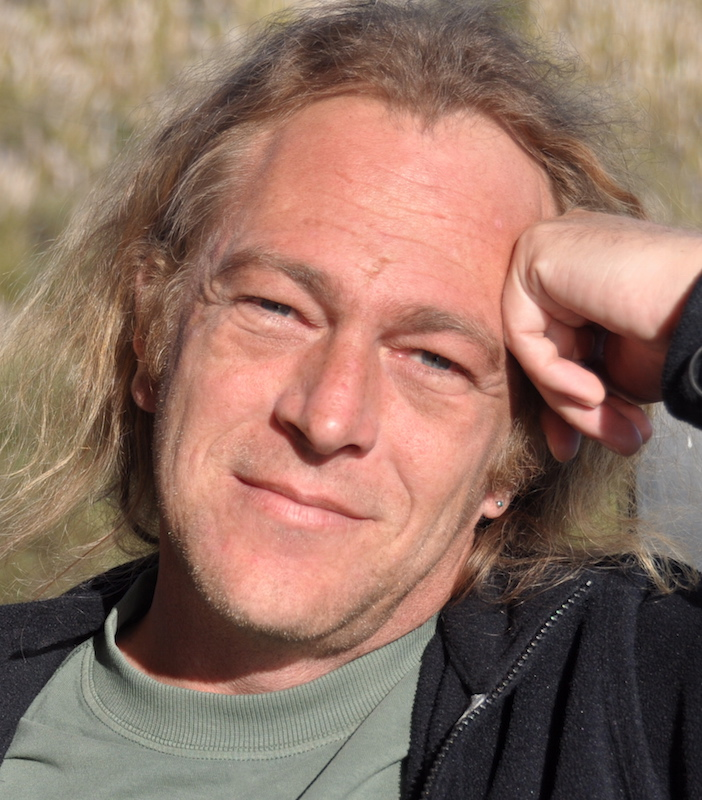
\includegraphics[width=3cm]{martin_small}\\
ORCID: 0000-0003-2366-382X
\end{tabular*}

\subsection*{Education}

\begin{tabular}{rl}
December 2010 & Habilitation at TU Vienna \\
April 2005   & PhD Degree in Computer Engineering with distinction from TU Vienna\\
1980 -- 1986 & Engineering School for Communications Engineering\\
              & and Electronics in St.\ P\"olten\\
\end{tabular}

\subsection*{Employment}
\begin{tabular}{rl}
 2020 & Guest Professor at TU Vienna\\
Since 2010    & Associate Professor at DTU Compute\\
2005 -- 2009 & Assistant Professor at the Institute of Computer Engineering, TU Vienna\\
Since 1994   & Self-employed with projects in automation and supervision\\
1992 -- 1994 & Software engineer at Wirtschafts- und Sozialwissenschaftliches Rechenzentrum\\
1987 -- 1991 & Software engineer at COIN Computerentwicklungen GmbH\\
1986 -- 1987 & Software engineer at SYSGRAPH Computergraphik GmbH\\
\end{tabular}

\subsection*{Summary of Scientific Work}

\begin{itemize}
  \item 28 journal articles
  \item 161 original, peer reviewed conference and workshop
      publications
  \item 4 books
  \item 1 patent
  \item 4701 citations, h-index of 37~\footnote{\url{http://scholar.google.com/citations?user=wiRNmwUAAAAJ&hl=en&oi=sra}}
  \item Supervised or co-supervised 11 PhD students and three Postdocs
  \item Reviewer for several journals and PC member of several
      conferences
  \item Member of the Expert Group for the Safety Critical Java
      Specification
  \item 5 research visits at University of California, Berkeley
  \item 13 Invited Talks and Tutorials on Chisel
\end{itemize}

\subsection*{Funding}

\begin{itemize}

\item 2020: High-Level Design and Verification of Digital Systems, InfinIT miniproject, DKK 180,000.-

\item 2016--2021: Time-predictable Control Systems (PREDICT),
Danish Council for Independent Research | Technology and Production
  Sciences under contract 6111-00363; DKK 5,170,177.-
  
  \item 2013--2016: Hard Real-Time Embedded Multiprocessor Platform - RTEMP
  (Co-applicant, PI is Jens Spars{\o}), 
  Danish Research Council for Technology and Production
  Sciences under contract 12-127600; DKK 4,977,862.-
  
  \item 2012--2016: ICT COST Action IC1202 Timing Analysis on Code-Level (TACLe),
  Co-applicant and work package 2 lead.
  
  \item 2011--2014: FP7 EC project T-CREST (Time-predictable
  Multi-Core Architecture for Embedded Systems) under grant
  agreement number 288008; EUR 3,807,000.- (total), EUR 703,000.- for DTU.
  I \textbf{led the funding proposal} and was \textbf{technical coordinator of T-CREST}.
  The proposal was \textbf{ranked at position 4 out of 59} submissions.
  
  \item 2011--2014: Certifiable Java for Embedded Systems (\emph{Principal Investigator} and funding applicant),
   Danish Research Council for Technology and Production
   Sciences under contract 10-083159; DKK 5,058,000.-.
   
  \item 2008--2010: FP7 EC project JEOPARD (Java Environment for
      Parallel Realtime Development) under grant agreement number
      216682; EUR 3,170,000.- (total), EUR 167,000.- for the TU
      Vienna. I wrote the proposal part for TU Vienna and I am
      lead the work package on architectures. JEOPARD
      deals with the issues for chip-multiprocessor solutions for
      real-time Java.
      
  \item 2004--2007: \emph{Principal Investigator} and funding
      applicant (self employed) for the national SME funding
      project: Implementation of the CLDC standard for real-time
      systems on a Java processor, EUR 80,000.-
      
\end{itemize}

\subsection*{Community Services}

   General chair ARCS 2019 in Copenhagen,
   EU projects track chair DATE 2019,
   Program chair JTRES 2009, 2016,
   Program chair WCET 2016,
   Program Co-Chair ISORC 2015,
   Workshop chair JTRES 2012 in Copenhagen,
   Track Co-Chair ACM SAC 2011,
   Editorial Board Member of Journal of Systems Architecture (JSA),
   Associate editor: EURASIP JES, IJERTCS,
   Guest editor for the special issue on \emph{Java,
      Technologies for Real-Time Distributed and Embedded,
      Systems} in Concurrency and Computation: Practice and,
      Experience,
   Workshop chair JTRES 2007 in Vienna,
   Expert Group member of the Safety Critical Java,
      Technology Specification (JSR 302),
   PC member JTRES 2006--2016,
   PC member FPL 2007--2015,
   PC member ACM SAC 2010--2022,
   PC member ISORC 2010, 2012--2022,
   PC member RTNS 2012, 2017,
   PC member WCET 2012, 2015--2019,
   PC member SIES 2016--2018,
   PC member SEUS 2010, 2013--2016,
   PC member Transact 2010,
   PC member PPPJ 2013, 2014, ECRTS WiP 2013,
   PC member SSV 2014,
   PC member HiRES 2014--2016,
   PC member Ada-Europe 2016,
   PC member RTSS 2018,
   PC member RTAS 2019,
   PC member DESTION 2019, 2020, 2021,
   PC member INDIN 2021,
   Reviewer for embedded systems journals: RTS, JSA, EURASIP JES,,
      TECS, TCAD, TII, TPDS, TCAS, SP\&E, IET Software, TPDS, S P\&E, IJERTCS, ESL, TAES,...

\end{document}
